\usetikzlibrary{calc}
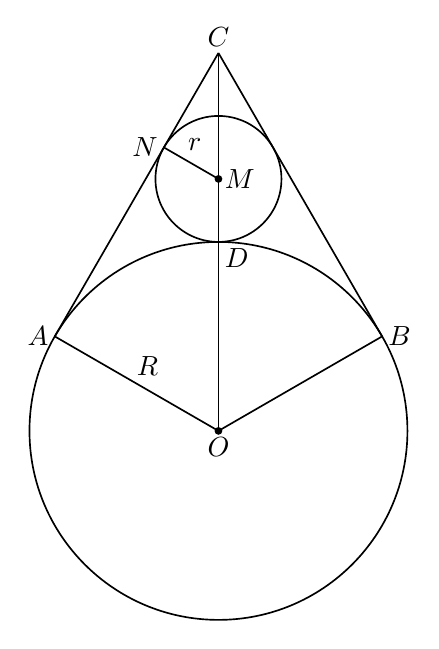
\begin{tikzpicture}[x=1cm,y=1cm,line width=.6pt,font=\normalsize]
\coordinate (O) at (0,0);
\coordinate (C) at (0,4.8);
\coordinate (M) at (0,3.2);
\coordinate (D) at (0,2.4);
\coordinate (A) at (-2.0785,1.2);
\coordinate (B) at (2.0785,1.2);
\coordinate (N) at (-0.6928,3.6);
\draw[solid] (O) circle[radius=2.4cm];
\draw[solid] (M) circle[radius=0.8cm];
\draw[solid] (C)--(A);
\draw[solid] (C)--(B);
\draw[solid] (C)--(O);
\draw[solid] (O)--(A);
\draw[solid] (O)--(B);
\draw[solid] (M)--(N);
\node[above=2pt,inner sep=0pt] at (C) {$C$};
\node[left=2pt,inner sep=0pt] at (A) {$A$};
\node[right=2pt,inner sep=0pt] at (B) {$B$};
\node[below=2pt,inner sep=0pt] at (O) {$O$};
\node[right=2pt,inner sep=0pt] at (M) {$M$};
\node[left=2pt,inner sep=0pt] at (N) {$N$};
\node[below right=2pt,inner sep=0pt] at (D) {$D$};
\node[anchor=center,inner sep=1pt] at (-0.90,0.82) {$R$};
\node[anchor=south,inner sep=1pt] at (-0.30,3.52) {$r$};

% Explicit named circle-center points, painted after all region fills.
\fill (O) circle[radius=1.4pt];
\fill (M) circle[radius=1.4pt];
\end{tikzpicture}
